\documentclass[border=16pt]{standalone}
\usepackage{tikz}
\usetikzlibrary{arrows.meta, positioning}
\begin{document}
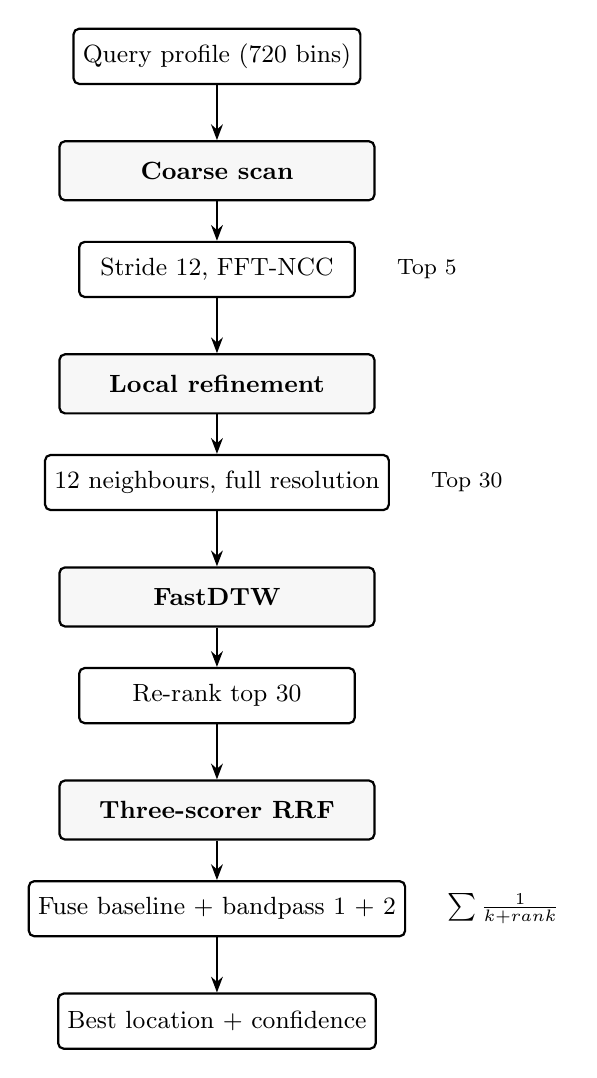
\begin{tikzpicture}[
    node distance=0.6cm and 1.0cm,
    box/.style={rectangle, draw=black, thick, minimum width=3.5cm, minimum height=0.7cm,
                text centered, font=\small, rounded corners=2pt},
    stage/.style={rectangle, draw=black, thick, minimum width=4.0cm, minimum height=0.75cm,
                  text centered, font=\small\bfseries, fill=gray!6, rounded corners=2pt},
    arr/.style={-{Stealth[length=2mm]}, thick},
]

% Input
\node[box] (q) {Query profile (720 bins)};

% Stage 1
\node[stage, below=0.7cm of q] (s1) {Coarse scan};
\node[box, below=0.5cm of s1] (s1d) {Stride 12, FFT-NCC};

% Stage 2
\node[stage, below=0.7cm of s1d] (s2) {Local refinement};
\node[box, below=0.5cm of s2] (s2d) {12 neighbours, full resolution};

% Stage 3
\node[stage, below=0.7cm of s2d] (s3) {FastDTW};
\node[box, below=0.5cm of s3] (s3d) {Re-rank top 30};

% RRF
\node[stage, below=0.7cm of s3d] (rrf) {Three-scorer RRF};
\node[box, below=0.5cm of rrf] (rrfd) {Fuse baseline + bandpass 1 + 2};

% Output
\node[box, below=0.7cm of rrfd] (out) {Best location + confidence};

% Arrows
\draw[arr] (q) -- (s1);
\draw[arr] (s1) -- (s1d);
\draw[arr] (s1d) -- (s2);
\draw[arr] (s2) -- (s2d);
\draw[arr] (s2d) -- (s3);
\draw[arr] (s3) -- (s3d);
\draw[arr] (s3d) -- (rrf);
\draw[arr] (rrf) -- (rrfd);
\draw[arr] (rrfd) -- (out);

% Side annotations
\node[font=\footnotesize, right=0.4cm of s1d] {Top 5};
\node[font=\footnotesize, right=0.4cm of s2d] {Top 30};
\node[font=\footnotesize, right=0.4cm of rrfd] {$\sum \frac{1}{k + \text{rank}}$};

\end{tikzpicture}
\end{document}
